% \begin{frame}{TITLE}
%     BODY
% \end{frame}

% To create a slide with a bullet list, use the following:
% \begin{frame}{TITLE}
%     \begin{itemize}
%         \item ITEM 1
%         \item ITEM 2
%     \end{itemize}    
% \end{frame}

% To create a slide with numbered list, use the following:
% \begin{frame}{TITLE}
%     \begin{enumerate}
%         \item ITEM 1
%         \item ITEM 2
%     \end{enumerate}
% \end{frame}

% To create a slide with a graphic:
% 1. Add the graphic to this folder (named picture.png)
% 2. Use the following:
% \begin{frame}{TITLE}
%     \centering
%     \includegraphics[height=0.7\textheight,width=0.7\textwidth,keepaspectratio]{picture.png}
% \end{frame}

% To create a slide with two columns, use the following:
% \begin{frame}{TITLE}
%     \begin{columns}
%         \begin{column}{0.5\textwidth}
%             COLUMN 1 BODY
%         \end{column}
%         \begin{column}{0.5\textwidth}
%             COLUMN 2 BODY
%         \end{column}
%     \end{columns}
% \end{frame}

\begin{frame}{Hardware Decisions}
    \begin{itemize}
        \item Single Board Computer: UP 7000 (Intel Processor N100, 8GB Mem, 64 GB Storage)
        \item GPS/Compass: SparkFun GPS Breakout - NEO-M9N, U.FL
        \item GPS Antenna: ACTPAT154 Active GPS Antenna
        \item Misc: 13.6v to 12v Voltage Regulator
    \end{itemize}
    \centering
    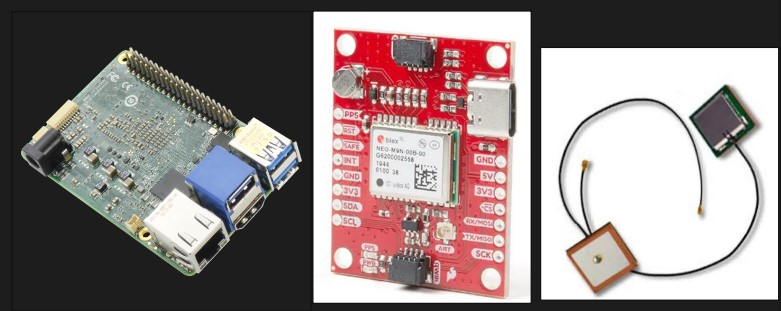
\includegraphics[height=0.5\textheight,width=0.5\textwidth,keepaspectratio]{images/rtt/Screenshot 2024-04-22 103014.jpg}
\end{frame}

\begin{frame}{Solar Panel Simulation}
    \centering
    \begin{columns}
        \begin{column}{0.5\textwidth}
            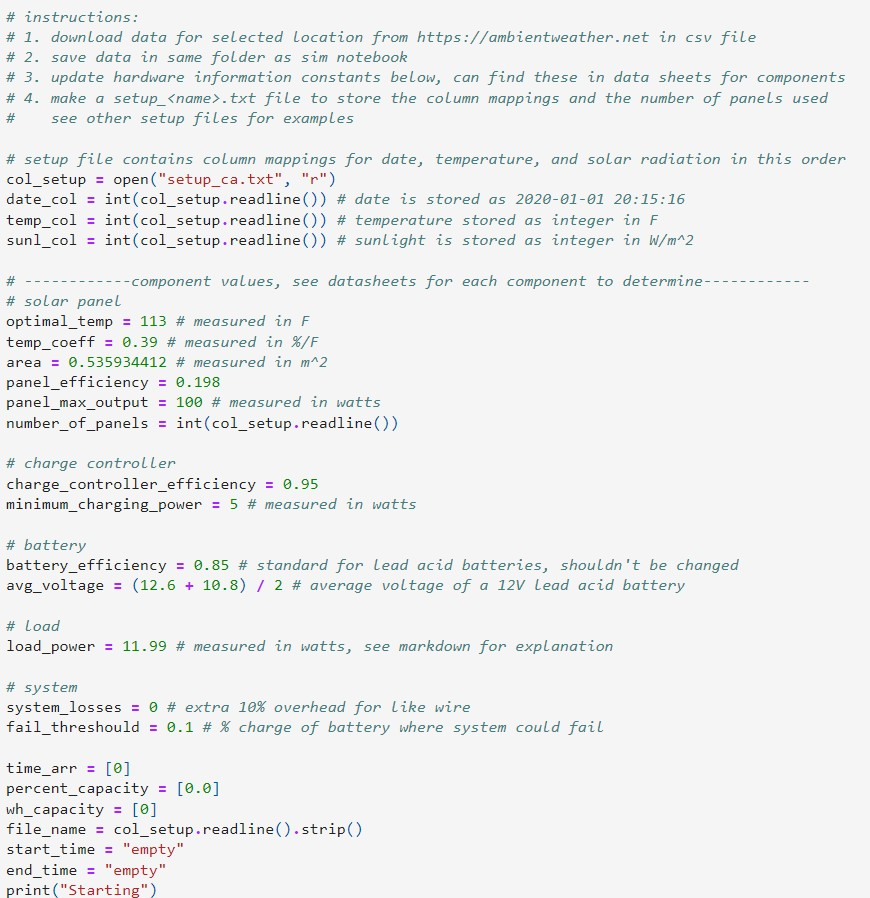
\includegraphics[height=1\textheight,width=1\textwidth,keepaspectratio]{images/rtt/Screenshot 2024-04-22 103941.jpg}
        \end{column}
        \begin{column}{0.5\textwidth}
            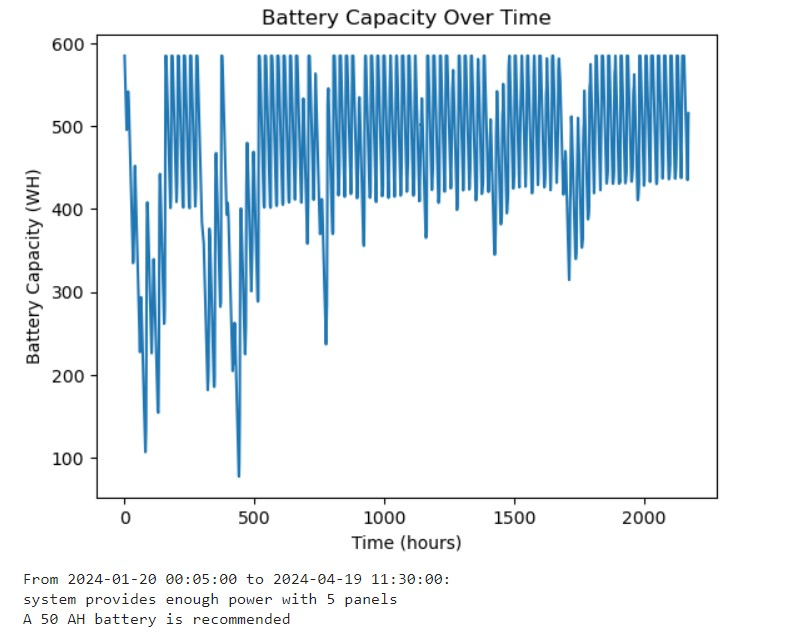
\includegraphics[height=1\textheight,width=1\textwidth,keepaspectratio]{images/rtt/Screenshot 2024-04-22 104426.jpg}
        \end{column}
    \end{columns}
\end{frame}
\begin{frame}{Other Work}
    \begin{itemize}
        \item PCB Work
        \item Tower Construction
        \item Location Estimation
    \end{itemize}
\end{frame}

